\documentclass[10pt,letterpaper]{article}
\usepackage[latin1]{inputenc}
\usepackage{amsmath}
\usepackage{amsfonts}
\usepackage{amssymb}
\usepackage{graphicx}
\usepackage[left=1.00in, right=1.00in, top=1.00in, bottom=1.00in]{geometry}
\usepackage{subfigure}
\begin{document}


\section{Describe the data you will analyze}
We will primarily be analyzing the CropScape\footnote{https://nassgeodata.gmu.edu/CropScape/} data from, United States Department of Agriculture
National Agricultural Statistics Service From 2008 - 2016. This is mainly satellite (raster) image data in which each pixel identifies a geographical area. The data has information like crop specific planting frequency per pixel, which is based on land cover information between the years 2008 and 2016. The data identifies the spatial distribution of multiple crops across the US through the last nine years. There are currently four individual crops for which complete data is available, these are: corn, cotton, soybeans, and wheat. In our study we will be focusing on the distribution of corn at the level of counties and use the Cropscape data as our ground truth. Below is the satellite image and the corresponding corn planting data for Montgomery county in 2016. 

\begin{figure}[ht]
\hfill
\subfigure{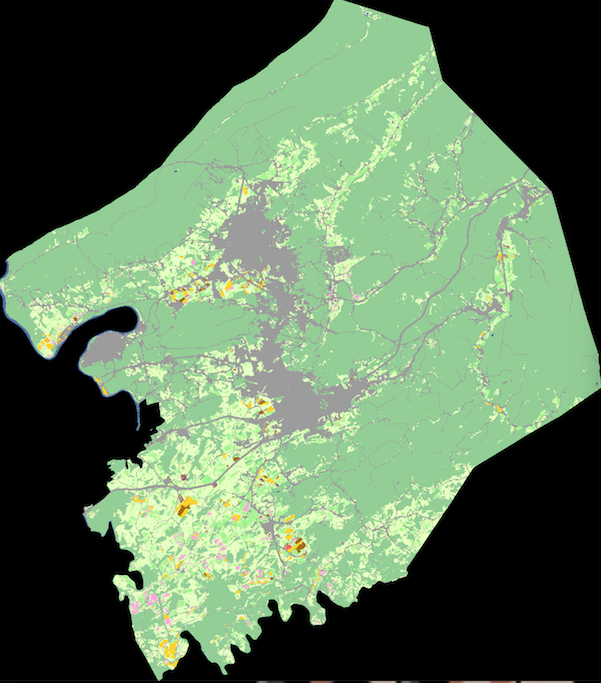
\includegraphics[width=5cm]{satellite.png}}
\hfill
\subfigure{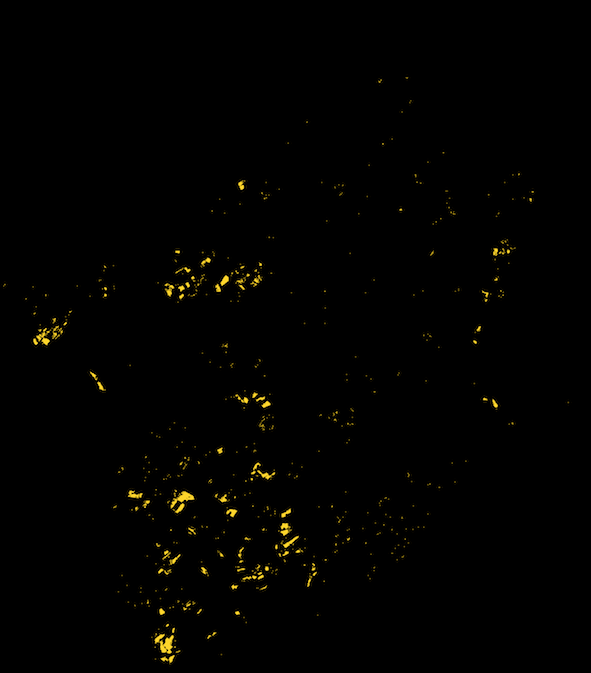
\includegraphics[width=5cm]{corn.png}}
\hfill \hfill
\caption{Sample satellite and corn cultivation image for Montgomery county}
\end{figure}

\noindent
Here, each of the yellow pixels in the image to the right represent that corn has been planted on the geographic location, for that pixel in 2016. 

\section{Describe at least one question you will answer using your analysis}


We will be answering the following three questions using our analysis:

\begin{enumerate}
	\item Given the satellite image of a county, can we predict how many pixels (acres of land) are present in that county on which corn is being grown?
	\item Can we accurately predict the distribution of crops (in particular corn) in a particular geographic area (county) of the United States?
	\item Can we augment the raster image data with additional freely available data for each pixel like: elevation (using something Google maps API), latitude, longitude, average annual temperature, average annual precipitation (rains+snow), distance from the sea, distance from the nearest water source, etc.? How does this impact the prediction accuracies?
\end{enumerate}

\noindent
This is not an exhaustive list, we might explore more questions if time permits. We would work on these questions in sequence, i.e. we will start with the first two questions and then work on the third question. 

\section{Describe the data analytics technique you will use to perform your analysis and why you think this technique will work well for your goal}

We will primarily be employing the following three techniques, however we might add others to this list if they seem to be useful:

\begin{enumerate}
	\item Support Vector Machine
	\item Ensemble methods (random forests, boosting, bagging, etc.)
	\item Neural Networks (deep learning)
\end{enumerate}

\section{Describe how you will evaluate whether the data analytics technique is successfully answering the question}

We will be using k-fold cross validation, and will evaluate our approach using:
\begin{enumerate}
	\item ROC curves
	\item Accuracy
	\item F-measure
\end{enumerate}

\section{List some references to existing work that is related or that your project will build on. Related work includes studies using the same data set, using a similar technical approach, or answering similar questions}

The following two papers are based on Cropland data, we will be using these for our first question and will be extending these for the last two questions:

\begin{enumerate}
	\item Shao, Yang, and Ross S. Lunetta. ``Comparison of support vector machine, neural network, and CART algorithms for the land-cover classification using limited training data points.'' ISPRS Journal of Photogrammetry and Remote Sensing 70 (2012): 78-87.
	\item Liu, Weiguo, Sucharita Gopal, and Curtis E. Woodcock. ``Uncertainty and confidence in land cover classification using a hybrid classifier approach.'' Photogrammetric Engineering \& Remote Sensing 70.8 (2004): 963-971.
\end{enumerate}


\section{List the members of your group.}

\begin{itemize}
	\item Meghendra Singh
	\item Arindam Fadikar
	\item Daniel Chen
\end{itemize}

\end{document}
